\section{Тригонометрия}

\subsection{Основные функции}

{\bold Единичной} называется окружность, которая задаётся урав"=нением $x^2+y^2=1$.\par

Тригонометрические функции соотносят {\ital координаты} точки единичной окружности
и {\ital градусную меру дуги}, образуемой ей с начальным радиусом.\par

{\bold Синус} --- нечётная функция с периодом $2\pi$; график --- {\ital синусоида}:
\\[-13pt]
% ---
$$\sin\colon\mathbb{R}\xrightarrow{\alpha\mapsto y}[-1;1]$$\\[-1pt]

Обратная нечётная функция к $\sin\vert_{[-\pi/2;\pi/2]}$ --- {\bold арксинус}:
% ---
$$\sin\trsp^{-1}=\arcsin\colon[-1;1]\xrightarrow{\alpha\mapsto y}[-\pi/2;\pi/2]$$
% ---
{\bold Косинус} --- чётная функция с периодом $2\pi$; график --- {\ital синусоида}
со смещением влево на $\pi/2$ {\ital\color{desc} («косинусоида»)}:\\[-6pt]
% ---
$$\cos\colon\mathbb{R}\xrightarrow{\alpha\mapsto x}[-1;1]$$\\[-1pt]

Обратная функция к $\cos\vert_{[0;\pi]}$ --- {\bold арккосинус}:
% ---
$$\cos^{-1}=\arccos\colon[-1;1]\xrightarrow{\alpha\mapsto x}[0;\pi]$$
% ---
{\bold Тангенс} --- нечётная функция с периодом $\pi$; график --- {\ital тангенсоида}:
\\[-13pt]
% ---
$$\tg\colon\mathbb{R}\backslash\{\pi/2+\pi n\mid n\in\mathbb{Z}\}\xrightarrow
{\alpha\mapsto y/x}\mathbb{R}$$\\[-1pt]

Обратная нечётная функция к $\tg\vert_{(-\pi/2;\pi/2)}$ --- {\bold арктангенс}:
% ---
$$\tg\trsp^{-1}=\arctg\colon\mathbb{R}\xrightarrow{y/x\mapsto\alpha}(-\pi/2;\pi/2)$$
% ---
{\bold Котангенс} --- нечётная функция с периодом $\pi$; график --- {\ital тангенсоида}
с симметрией относительно оси $Ox$ и смеще"=нием вправо на $\pi/2$ {\ital\color{desc} 
(«котангенсоида»)}:\\[-7pt]
% ---
$$\ctg\colon\mathbb{R}\backslash\{\pi n\mid n\in\mathbb{Z}\}\xrightarrow{\alpha\mapsto
x/y}\mathbb{R}$$\\[-1pt]

Обратная функция к $\ctg\vert_{(0;\pi)}$ --- {\bold арккотангенс}:
% ---
$$\ctg\trsp^{-1}=\arcctg\colon\mathbb{R}\xrightarrow{x/y\mapsto\alpha}(0;\pi)$$

\subsection{Основные тождества}

Из определений тригонометрических функций следует:

\begin{tabularx}{\textwidth}{C@{\quad\quad}C}
$\begin{aligned}
\sin^2\alpha+&\cos^2\alpha=1\\
1+\tg^2\alpha&=1/\cos^2\alpha\\
1+\ctg^2\alpha&=1/\sin^2\alpha
\end{aligned}$ &
$\begin{aligned}
\arccos x&=\arcsin(\sqrt{1-x^2})\\
\arccos x&=(\sqrt{1-x^2}/x)\\
\arcsin y&=\arcctg(\sqrt{1-y^2}/y)
\end{aligned}$
\end{tabularx}

\vspace*{-6pt}
\subsection{Сумма и разность двух углов}

Из скалярного произведения векторов следует:
% ---
\begin{align*}
\cos(\alpha\pm\beta)&=\cos\alpha\cos\beta\mp\sin\alpha\sin\beta\\
\sin(\alpha\pm\beta)&=\sin\alpha\cos\beta\pm\sin\beta\cos\alpha
\end{align*}\leavevmode\\[-10pt]
% ---
\begin{tabularc}{0pt}{0pt}{c @{\quad\quad} c}{c}
\parbox{144pt}{$$\tg(\alpha\pm\beta)=\frac{\tg\alpha\pm\tg\beta}{1\mp\tg\alpha\tg\beta}
$$} &
\parbox{150pt}{$$\ctg(\alpha\pm\beta)=\frac{\ctg\alpha\ctg\beta\mp 1}{\ctg\alpha\pm
\ctg\beta}$$}
\end{tabularc}
% ---
{\bold Доказательство.} Пусть $\vec{A}=\langle\cos\alpha;\sin\alpha\rangle,\ 
\vec{B}=\langle\cos\beta;\sin\beta\rangle$.\par

Рассмотрим их скалярное произведение:
% ---
$$+\begin{cases}
\vec{A}\cdot\vec{B}=\cos\alpha\cos\beta+\sin\alpha\sin\beta\\
\vec{A}\cdot\vec{B}=\norm{\vec{A}}\ \norm{\vec{B}}\cos(\alpha-\beta)=\cos(\alpha-\beta)
\end{cases}\hspace*{-12pt}\implies$$
% ---
$$\cos(\alpha-\beta)=\cos\alpha\cos\beta+\sin\alpha\sin\beta\qedw$$
% ---
Затем полезно применить эти четыре формулы:
% ---
\begin{align*}
\alpha+\beta&=\alpha-(-\beta)\\
\sin(\alpha-\beta)&=\cos((\pi/2-\alpha)+\beta)
\end{align*}
$$\tg\alpha=\sin\alpha/\cos\alpha\quad\quad\ctg\alpha=\cos\alpha/\sin\alpha\qedb$$

\subsection{Двойной угол}

Из формул суммы и разности двух углов следует:\par
% ---
\vspace*{-6pt}
\begin{tabularc}{0pt}{0pt}{c @{\quad\quad} c}{c}
\parbox{125pt}{$$\cos 2\alpha=\cos^2\alpha-\sin\trsp^2\alpha$$} &
\parbox{114pt}{$$\sin 2\alpha=2\sin\alpha\cos\alpha$$}\\[-6pt]
\parbox{95pt}{$$\tg 2\alpha=\frac{2\tg\alpha}{1-\tg\trsp^2\alpha}$$} &
\parbox{106pt}{$$\ctg 2\alpha=\frac{\ctg\trsp^2\alpha-1}{2\ctg\alpha}$$}
\end{tabularc}\leavevmode\\[-23pt]
% ---
$$(\sin\alpha\pm\cos\alpha)^2=1\pm\sin 2\alpha$$

\subsection{Формулы приведения}

\begin{column*}{r}{78mm}
Из формул суммы и разности двух углов следуют {\ital формулы приведения}, которые
имеют вид:
% ---
$$f(\pi n/2\pm\alpha)={\color{desc}\pm co}f(\alpha),\ n\in\mathbb{Z}$$
% ---
Конечная функция и её знак опреде"=ляются по графику; стрелками обозна"=чены места
смены функции на~{\ital кофункцию}.
\end{column*}
% ---
\begin{column*}{r}{124pt}
{\centering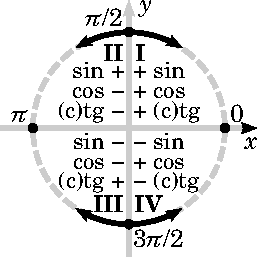
\includegraphics{drawing.pdf}\par}
\end{column*}

{\bold Следствие.} Для обратных функций верно:

\begin{tabularx}{\textwidth}{C@{\quad\quad}C}
$\begin{aligned}
\arcsin x+\arccos x&=\pi/2\\
\arctg x+\arcctg x&=\pi/2
\end{aligned}$ &
$\begin{aligned}
\arccos x+\arccos(-x)&=\pi\\
\arcctg x+\arcctg(-x)&=\pi
\end{aligned}$
\end{tabularx}

\subsection{Формулы понижения степени}

Из формул двойного угла и основного тригонометрического тождества следует:\par
% ---
\begin{tabularc}{0pt}{0pt}{c @{\quad\quad} c}{c}
$\begin{aligned}
\cos^2\frac{\alpha}{2}&=\frac{\cos\alpha+1}{2}\\
\sin\trsp^2\frac{\alpha}{2}&=\frac{1-\cos\alpha}{2}
\end{aligned}$ &
$\begin{aligned}
\tg\trsp^2\frac{\alpha}{2}&=\frac{1-\cos\alpha}{\cos\alpha+1}\\
\ctg\trsp^2\frac{\alpha}{2}&=\frac{1-\cos\alpha}{\cos\alpha+1}
\end{aligned}$
\end{tabularc}

Из них легко выводятся формулы {\ital половинного угла}.

\subsection{Сумма и разность двух функций}

Из формул суммы и разности двух углов следует:
% ---
\begin{align*}
\sin\alpha\pm\sin\beta&=2\sin\frac{\alpha\pm\beta}{2}\cos\frac{\alpha\mp\beta}{2}\\[-2pt]
\cos\alpha+\cos\beta&=2\cos\frac{\alpha+\beta}{2}\cos\frac{\alpha-\beta}{2}\\[-2pt]
\cos\alpha-\cos\beta&=-2\sin\frac{\alpha+\beta}{2}\sin\frac{\alpha-\beta}{2}\\
\end{align*}\\[-34pt]
% ---
$$a\sin\alpha+b\cos\alpha=c\sin(\alpha+\phi)=c\cos(\alpha-\phi),\ c=\sqrt{a^2+b^2}$$
% ---
Из них можно вывести формулы {\ital произведения двух функций}.

{\bold Доказательство.} Рассмотрим сумму синусов:
% ---
$$\sin(x+y)+\sin(x-y)=$$
$$\sin x\cos y+\sin y\cos x+\sin x\cos y-\sin y\cos x=2\sin x\cos y$$
% ---
Введём обозначения:
% ---
$$\begin{cases}
x+y=\alpha\\
x-y=\beta
\end{cases}\hspace*{-12pt}\iff
\begin{cases}
2x=\alpha+\beta\\
2y=\alpha-\beta
\end{cases}\hspace*{-12pt}\iff
\begin{cases}
x=\frac{\alpha+\beta}{2}\\
y=\frac{\alpha-\beta}{2}
\end{cases}$$
% ---
Таким образом,
% ---
$$\sin\alpha+\sin\beta=2\sin\frac{\alpha+\beta}{2}\cos\frac{\alpha-\beta}{2}.\qedw$$
% ---
Похожие формулы доказываются аналогично.$\qedw$\par

Рассмотрим синус суммы двух углов:
% ---
$$c\sin(\alpha+\phi)=c\sin\alpha\cos\phi+c\sin\phi\cos\alpha$$
% ---
Обозначим $a=c\cos\phi$, $b=c\sin\phi$ и найдём сумму квадратов:
% ---
$$a^2+b^2=c^2(\sin\trsp^2\phi+\cos^2\phi)=c^2\iff c=\sqrt{(a^2+b^2)}\qedw$$
% ---
Случай с косинусом доказывается аналогично.$\qedb$

\subsection{Подстановка Вейерштрасса}

Тригонометрические функции от $\alpha$ можно выразить через тангенс от $\alpha/2$
{\ital\color{desc}(К. Вейерштрасс)}:
% ---
$$\sin\alpha=\frac{2\tg\frac{\alpha}{2}}{1+\tg\trsp^2\frac{\alpha}{2}}\quad\quad
\cos\alpha=\frac{1-\tg\trsp^2\frac{\alpha}{2}}{1+\tg\trsp^2\frac{\alpha}{2}}$$
% ---
{\bold Доказательство.} Распишем каждую функцию:
% ---
$$\sin\alpha=\frac{2\sin\frac{\alpha}{2}\cos\frac{\alpha}{2}}{\sin\trsp^2\frac{\alpha}{2}
+\cos^2\frac{\alpha}{2}}=\frac{2\tg\frac{\alpha}{2}}{1+\tg\trsp^2\frac{\alpha}{2}}\qedw$$
$$\cos\alpha=\frac{\cos^2\frac{\alpha}{2}-\sin\trsp^2\frac{\alpha}{2}}{\sin\trsp^2\frac
{\alpha}{2}+\cos^2\frac{\alpha}{2}}=\frac{1-\tg\trsp^2\frac{\alpha}{2}}{1+\tg\trsp^2\frac
{\alpha}{2}}\qedb$$
